\pdfminorversion=4
\documentclass[xcolor=dvipsnames,hyperref={pdfpagelabels=false},handout,unknownkeysallowed]{beamer}
\usepackage{tabls}
\usepackage{graphicx}
\usepackage{subcaption}
%\usepackage{animate}




%Load the myriad packages
\usepackage{xcolor}
\usepackage{tikz}
\usetikzlibrary{shapes.geometric, arrows}
\tikzstyle{startstop} = [rectangle, rounded corners, minimum width=2cm, text
    width=1.8cm, minimum height=1cm,text centered, text=white,draw=black, fill=Gray!140]
\tikzstyle{io} = [trapezium, trapezium left angle=70, trapezium right angle=110,
minimum width=0.5cm, minimum height=1cm, text centered, draw=black,
fill=blue!20!Gray!90!,text=white]
\tikzstyle{process} = [rectangle, minimum width=2cm, minimum height=1cm, text
centered, text width=2cm, draw=black, text=white,fill=Gray!140!blue!70!white]
\tikzstyle{decision} = [diamond, minimum width=2.0cm, minimum
    height=0.81cm,aspect=1.40, text centered, draw=black, fill=Gray!,text=white]
\tikzstyle{arrow} = [thick,line width=0.5mm,->,>=stealth]
\tikzstyle{arrow1} = [dashed,->,>=stealth]

\setbeamertemplate{navigation symbols}{}%remove navigation symbols
\useoutertheme{infolines}

%\definecolor{myblue}{rgb}{0.7, 0.7, 60.0}
\definecolor{mylightblue}{rgb}{1,1,1}
\newcommand*{\boxedcolor}{blue}
\makeatletter
\renewcommand{\boxed}[1]{\textcolor{\boxedcolor}{%
  \fbox{\normalcolor\m@th$\displaystyle#1$}}}
\makeatother

\renewcommand{\u}[1]{\underline{#1}}

\newcommand{\iso}[2]{${}^{{#2}}${#1} }
\newcommand{\nubar}[0]{$\overline{\nu}$ }
\newcommand{\keff}[0]{\ensuremath{{k}_{\textsf{eff}}} }
\newcommand{\expect}[1]{E[#1] }
\newcommand{\colg}[1]{{\color{ForestGreen} #1}}
\newcommand{\coly}[1]{{\color{yellow} #1}}
\newcommand{\colb}[1]{{\color{blue} #1}}
\newcommand{\colr}[1]{{\color{red} #1}}
\usepackage{amsfonts}
\newlength{\wideitemsep}
\setlength{\wideitemsep}{8pt}
%\addtolength{\wideitemsep}{5pt}
\let\olditem\item
\renewcommand{\item}{\setlength{\itemsep}{\wideitemsep}\olditem}

\newcommand{\N}{\mathbb{N}}
\newcommand{\Z}{\mathbb{Z}}
\newcommand{\deriv}[2]{\frac{\mathrm{d} #1}{\mathrm{d} #2}}
\newcommand{\pderiv}[2]{\frac{\partial #1}{\partial #2}}
\newcommand{\bx}{\mathbf{X}}
\newcommand{\ba}{\mathbf{A}}
\newcommand{\by}{\mathbf{Y}}
\newcommand{\bj}{\mathbf{J}}
\newcommand{\bs}{\mathbf{s}}
\newcommand{\B}[1]{\ensuremath{\mathbf{#1}}}
\newcommand{\Dt}{\Delta t}
\renewcommand{\d}{\mathsf{d}}
\newcommand{\mom}[1]{\langle #1 \rangle}
\newcommand{\cur}[1]{\left\{ #1 \right\}}
\newcommand{\xl}{{x_{i-1/2}}}
\newcommand{\xr}{{x_{i+1/2}}}
\newcommand{\il}{{i-1/2}}
\newcommand{\ir}{{i+1/2}}

%The next lines automatically add outline slides at start of each section
\AtBeginSection[]
{
    \begin{frame}<*>
        \frametitle{Outline}
        \tableofcontents[currentsection,currentsubsection]
    \end{frame}
}


\setbeamerfont{frametitle}{size=\large}
\setbeamerfont{normal font}{size=\tiny}

\graphicspath{{figures/}}

\usepackage{verbatim}
\usepackage{comment}
\usepackage[]{datetime}
\usepackage{multirow}
\newcommand{\thedate}{\today}


%\addtobeamertemplate{navigation symbols}{}{ %
%    \usebeamerfont{footline}%
%    \usebeamercolor[fg]{footline}%
%    \insertframenumber/\inserttotalframenumber
%}


% HACKING IN page numbers
%
%    \expandafter\def\expandafter\insertlogo\expandafter{%
%        \insertlogo\hspace{4pt}%
%        \raisebox{-6.9pt}{\scriptsize{\insertframenumber\,/\,\inserttotalframenumber}}}

\setlength{\tabcolsep}{1.05cm}

%Aggie-themed
\pgfdeclareimage[height=0.1in]{TAMUlogo}{tamu_engineering.png}
\logo{\raisebox{-8pt}{\pgfuseimage{TAMUlogo}}}
\titlegraphic{\centering\begin{tabular}{lr}
\includegraphics[trip=4.0in 0.0in 0.0in 0.0in,clip,height=0.18\textheight]{NEUP.jpg} &

\includegraphics[height=0.18\textheight]{tamu_seal.png}\end{tabular}}
%Michigan-themed
%\pgfdeclareimage[height=0.1in]{UMlogo}{michigan_engineering.png}
%\logo{\raisebox{-8pt}{\pgfuseimage{UMlogo}}}
%\titlegraphic{
\includegraphics[height=0.2\textheight]{michigan_block_m.png}}


%%%%%%%%%%%%%%%%%%%%%%%%%%%%%%%%%%%%%%%%%%%%%%%%%%%%%%%%%%%%%%%
% Optional packages, used to show off certain tricks

\newlength \figwidth
\setlength \figwidth {0.5\textwidth}

\setlength{\leftmargin}{-2cm}
\setlength{\rightmargin}{-2cm}

%%%%%%%%%%%%%%%%%%%%%%%%%%%%%%%%%%%%%%%%%%%%%%%%%%%%%%%%%%%%%%%

\usepackage[english]{babel}
\usetheme{Frankfurt}

%Make it Aggie Maroon
\usecolortheme[RGB={80,0,0}]{structure}  
%Or Michigan Blue
%\usecolortheme[RGB={0,0,153}]{structure}  
%Or Michigan Maize
%\usecolortheme[RGB={255,204,0}]{structure}  

  % This will typeset only the frames (or slides) that have the given label ("current" in this case).

\title[HOLO for TRT]{A High-Order Low-Order Algorithm with Exponentially-Convergent Monte Carlo for
    Thermal Radiative Transfer}
    \author[S.R. Bolding]{{\large Simon Bolding\inst{1}, Jim Morel\inst{1}, and Mathew Cleveland\inst{2}}}
    \institute[]{{\large \inst{1} Texas A\&M University\\ \inst{2} Los Alamos National Laboratory}}
\date{{MC 2015 - April 22} }
\subject{}
%\institute{Los Alamos National Laboratory}

% \classificationlevel{SECRET/RD}
% \transmissible{}

%\reportnum{\textcolor{blue}{SAMPLE TEMPLATE ONLY \\ Contains NO Classified
%Information}}

% \dissableframenumber
\begin{document}

\begin{frame}
    \titlepage \vspace{-0.213in}
    \begin{center}
    \end{center}    
\end{frame}

\setlength{\tabcolsep}{6pt}

\begin{frame}
\frametitle{Outline}
\begin{minipage}{0.061\linewidth}
\hfill                      
\end{minipage}
\begin{minipage}{0.8\linewidth}
\tableofcontents[
hideothersubsections,
sectionstyle=show,
subsectionstyle=hide
]
\end{minipage}

\end{frame}


\section{Introduction}
\subsection{}

%%%%%%%%%%%%%%%%%%%%%%%%%%%%%%%%%%%%%%%%%%%%%%%%%%%%%%%%%%%%%%%%%%%%%%%%%%%%%%%%%%%%%%%%%
\begin{frame}
\frametitle{Overview}
\begin{itemize}
\item We are interested in modeling thermal radiation transport in the High-Energy Density Physics regime.
\begin{itemize}
\item Temperatures on order of $10^6$ K or more.  
\item Significant energy and momentum may be exchanged with material.
\end{itemize}\pause
\item Radiative transfer simulations important in modeling: 
\begin{itemize}
\item Material under extreme conditions
\item Inertial confinement fusion
\item Supernovae and other astrophysical phenomena.
\end{itemize}
\end{itemize}
\end{frame}


%%%%%%%%%%%%%%%%%%%%%%%%%%%%%%%%%%%%%%%%%%%%%%%%%%%%%%%%%%%%%%%%%%%%%%%%%%%%%%%%%%%%%%%%%
\begin{frame}
\frametitle{The gray thermal radiative transfer equations}
\begin{itemize}
\item The 1D, frequency-integrated (grey) equations
\begin{align*}\label{ho_cont}
    \frac{1}{c}\pderiv{I}{t} + \mu \pderiv{I}{x} + \sigma_t I(x,\mu)
&= \frac{1}{2} \sigma_a a c T^4,
  \\
  C_v \pderiv{T}{t} &=  \sigma_a \phi(x) - \sigma_a a c T^4, \\
   \phi(x) &= \int_{-1}^1 I(x,\mu) \d \mu.
\end{align*}
        \item Fundamental unknowns are the radiation intensity $I(x,\mu)$ and material
            temperature $T$
        \item \pause Absorption cross section ($\sigma_a$) can be a strong function of $T$
        \item Equations are nonlinear and may be tightly coupled 
\end{itemize}

\end{frame}

%%%%%%%%%%%%%%%%%%%%%%%%%%%%%%%%%%%%%%%%%%%%%%%%%%%%%%%%%%%%%%%%%%%%%%%%%%%%%%%%%%%%%%%%%
\begin{frame}
\frametitle{The Implicit Monte Carlo Method}
\begin{itemize}
\item Equations often solved with Monte Carlo (MC) via the Implicit Monte Carlo (IMC) method
\item In IMC, the material energy equation is linearized over a time step and eliminated from the system
    \begin{itemize}
        \item Results in effective emission and scattering terms
\item This linear transport equation is solved with standard MC particle transport
    algorithms
\item Continuous integration in time
    \end{itemize}
\item Drawbacks 
\begin{itemize}
\item Effective scattering cross section can be very large 
\item Nonlinearities not converged
\item Reconstruction of linear source shape in cell
\end{itemize}
\end{itemize}
\end{frame}

%%%%%%%%%%%%%%%%%%%%%%%%%%%%%%%%%%%%%%%%%%%%%%%%%%%%%%%%%%%%%%%%%%%%%%%%%%%%%%%%%%%%%%%%%
\begin{frame}
    \frametitle{An alternative  High-Order Low-Order approach}
    {\small
        \begin{itemize}
            \item[]<1-> \begin{block}{Basic Idea} Build a low-order (LO) system that can be efficiently solved,
                with high-order (HO) correction from simpler MC simulations \end{block}
                \vspace{-0.321in}
              \item<1-> The LO system, formed over a fixed spatial finite element
                  (FE) mesh, contains \colb{angular consistency terms}.
              \item<2-> The LO solver resolves non-linear temperature dependence with
                  Newtons method
                \begin{itemize}
                    \item<2-> \colb{Lower dimensional} problem in angular variable
                    \item<2-> Produces a linear-discontinuous (LD) finite element  representation of sources
                  %  \item Consistency terms derived directly from transport equation
                \end{itemize}
                \vspace{-0.1in}
            \item<3-> The HO system is a fixed-source, pure-absorber transport problem
                \begin{itemize}
                    \item No effective scattering events
                    \item Solved with ECMC for efficient reduction of statisical noise 
                \end{itemize}
        \end{itemize}
    }
\end{frame}




\begin{frame}
    \frametitle{High-Order Low-Order Algorithm}
    %\fontsize{9}{5.0}\selectfont
        \resizebox{0.99\linewidth}{!}{
    \fontsize{10}{12.0}\selectfont
    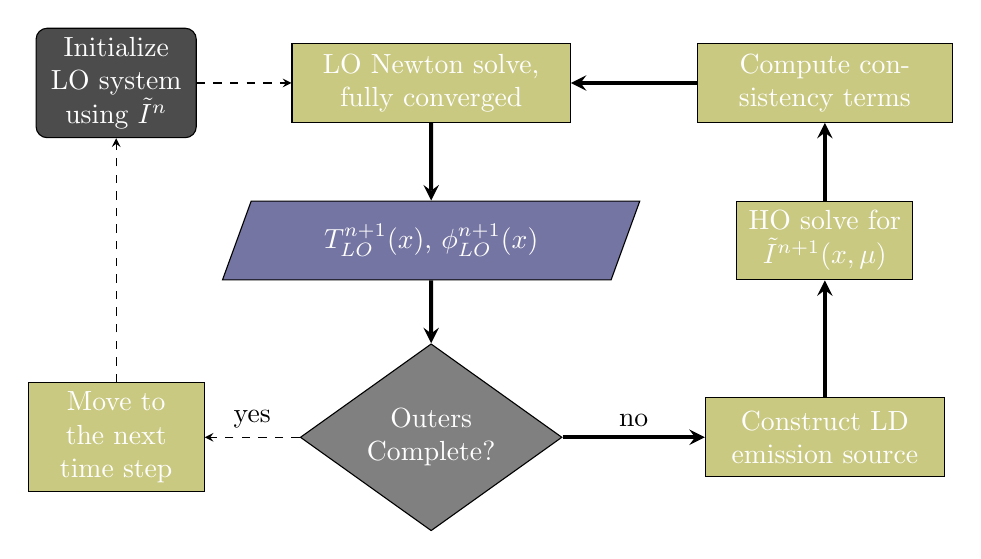
\begin{tikzpicture}[node distance=2cm]
        \node (start) [startstop] {Initialize LO system using $\tilde{I}^n$};
        \node (in1) [process, right of=start, xshift=2cm, text width=3.3cm]  {
        {LO Newton solve, fully converged}};%{LO solve:\vspace{0.041in}        $\B D(\mu^{HO})\Phi = \frac{1}{\keff}\B F\Phi$};
        \node (pro1) [io, below of=in1] {$T_{LO}^{n+1}(x)$, $\phi_{LO}^{n+1}(x)$};
        \node (dec1) [decision, below of=pro1, yshift=-0.5cm, text width=1.74cm] {Outers Complete?};
        \node (pro2a) [process, left of=dec1, xshift=-2.0cm] {Move to the next time step};
        \node (srcs) [process, right of=dec1, xshift=3.0cm, text width=2.8cm] {
        {Construct LD emission source}};
        \node (pro2b) [process, above of=srcs, yshift=0.5cm] {{HO solve
        for $\tilde I^{n+1}(x,\mu)$}};
        \node (cons) [process, above of=pro2b, text width=3.0cm] {{Compute consistency
        terms}};
        \draw [arrow1] (start) -- (in1);
        \draw [arrow] (in1) -- (pro1);
        \draw [arrow] (pro1) -- (dec1);
        \draw [arrow] (srcs) -- (pro2b);
        \draw [arrow] (dec1.east) -- node[anchor=south] {no} (srcs);
        \draw [arrow1] (dec1.west) -- node[anchor=south] {yes} (pro2a);
        \draw [arrow1] (pro2a) -- (start);
        \draw [arrow] (pro2b) -- (cons);
        \draw [arrow] (cons) -- (in1);
    \end{tikzpicture}
}
\end{frame}



\section{Low-Order Solver}
\subsection{}


%%%%%%%%%%%%%%%%%%%%%%%%%%%%%%%%%%%%%%%%%%%%%%%%%%%%%%%%%%%%%%%%%%%%%%%%%%%%%%%%%%%%%%%%%
\begin{frame}
    \frametitle{LO Discretization \& Space-Angle Moments}
    \begin{itemize}
        \item Backward Euler discretization in time
        \item Linear discontinuous (LD) FE in space for $\phi$, $T$, and $T^4$   \end{itemize}
    \begin{centering}
        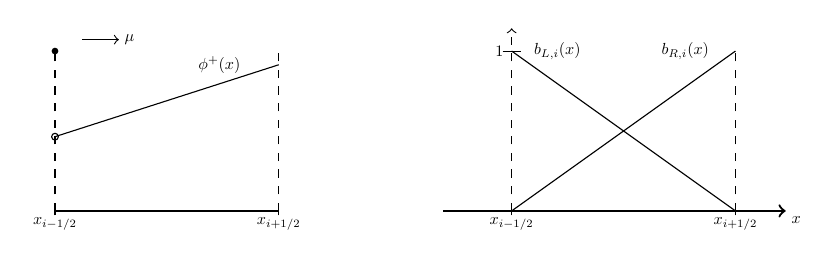
\begin{tikzpicture}[scale=0.58, every node/.style={transform shape}]
            \draw (1.0,4.0) node[fill,circle,inner sep=0pt,minimum
            size=4.2pt] {};
            \filldraw[color=black, fill=white] (1,2.1250) circle (2.1pt);
            \draw [->] (1.6,4.25) -- (2.4,4.25) node[anchor=west] {$\mu$};
            \draw (1.0,0.4) -- (1.0,0.6) node[below, pos=0.4] {$x_{i-1/2}$};
            \draw (5.90,0.4) -- (5.90,0.6) node[below, pos=0.4] {$x_{i+1/2}$};
            \node at (4.6,3.70) {$\phi^+(x)$};
            \draw [thick] (1.0,0.5) -- (5.9,0.5) node[anchor=north west] {};
            \draw (1.0,2.125) -- (5.90,3.70);
            \draw [dashed] (5.90,0.5) -- (5.90,4);
            \draw [dashed] (1.0,0.5) -- (1.0,4);

            \draw (10.8,4.0) -- (11.2,4.0) node[anchor=east]{$1$ \hspace{0.4em} };
            \draw (11.0,0.4) -- (11.0,0.6) node[below, pos=0.4] {$x_{i-1/2}$};
            \draw (15.90,0.4) -- (15.90,0.6) node[below, pos=0.4] {$x_{i+1/2}$};
            \node at (14.8,4.0) {$b_{R,i}(x)$};
            \node at (12.0,4.0) {$b_{L,i}(x)$};
            \draw [thick,->] (9.5,0.5) -- (17.0,0.5) node[anchor=north west] {$x$};
            \draw [dashed,-] (15.90,0.5) -- (15.90,4);
            \draw [dashed,->] (11.0,0.5) -- (11.0,4.5);
            \draw (11.0,0.5) -- (15.90,4.0);
            \draw (15.90,0.5) -- (11.0,4.0);
        \end{tikzpicture}
    \end{centering}
    \begin{itemize}
        \item Half-range integrals in angle
\item \emph{Examples} of moments:
    \end{itemize}
    \begin{center}
    \begin{tabular}{cc}
        \underline{Spatial: left basis} & \underline{Angular: positive flow} \\ 
        $ {\displaystyle \mom{\cdot}_{L,i} = \frac{2}{h_i} \int_{x_\il}^{x_\ir}
        b_{L,i}(x)(\cdot) \d x \quad }$  & ${ \quad \displaystyle \phi^+(x) = 2\pi\int_0^1 \psi(x,\mu) \d \mu}$
    \end{tabular}
    \end{center}

\end{frame}


%%%%%%%%%%%%%%%%%%%%%%%%%%%%%%%%%%%%%%%%%%%%%%%%%%%%%%%%%%%%%%%%%%%%%%%%%%%%%%%%%%%%%%%%%
\begin{frame}
    \frametitle{Forming the LO System}
    \begin{itemize}
    \item Backward Euler discretization in time
    \item We take half range angular integralsspatial and angular moments of the equations to reduce
        dimensionality.
    \item Taking moments of T.E. yields 4 radiation equations, and 2 material energy
        equations, per cell

    \item Conserves the total energy in the system

    \item Cell unknowns: $\mom{\phi}_{L,i}^{n+1,+}$, $\mom{\phi}_{R,i}^{n+1,+}$,
        $\mom{\phi}_{L,i}^{n+1,-}$, $\mom{\phi}_{R,i}^{n+1,-}$, $T_{L,i}$, $T_{R,i}$

    \end{itemize}
\end{frame}


%%%%%%%%%%%%%%%%%%%%%%%%%%%%%%%%%%%%%%%%%%%%%%%%%%%%%%%%%%%%%%%%%%%%%%%%%%%%%%%%%%%%%%%%%
\begin{frame}
    \frametitle{Computing LO Consistency terms from HO Solution}
    \begin{itemize}
        \item The streaming operator contains generally unknown weighted angular averages,
            called \colb{consistency terms}
        \item For $\mu>0$, $L$ moment
    \begin{equation}
\mom{{\mu}}_{L,i}^{+} \simeq \frac{\displaystyle 
\frac{2}{h_i} \int\limits_0^1 \int\limits_\xl^\xr \mu \, b_{L,i}(x) \tilde I^{HO}(x,\mu) \d \mu \d x } 
{\displaystyle \frac{2}{h_i} \int\limits_0^1 \int\limits_\xl^\xr \, b_{L,i}(x)
\tilde I^{HO}(x,\mu) \d \mu \d x } 
    \end{equation}
        \item ECMC gives LDFE $\tilde  I^{HO}(x,\mu)$ for computing terms directly
    \end{itemize}
\end{frame}



\section{High-Order Solver}
\subsection{}



%%%%%%%%%%%%%%%%%%%%%%%%%%%%%%%%%%%%%%%%%%%%%%%%%%%%%%%%%%%%%%%%%%%%%%%%%%%%%%%%%%%%%%%%%
\begin{frame}
    \frametitle{Overview of Exponentially Convergent Monte Carlo}
    \begin{itemize}
        \item Iterative form of residual Monte Carlo
      \begin{itemize}
          \item Each batch tallies the \colb{error} in current estimate of solution, which
            is a transport problem with a reduced source
    \item Can reduce statistical error \colb{globally} $\propto e^{-\alpha N}$
           \item In TRT problems, old angular intensity provides a very good guess of new
               solution, significantly reducing the required number of histories
\end{itemize}
     \end{itemize}
    \begin{minipage}{0.6\linewidth}
        \vspace{-2.0in}
     \begin{itemize}
        \item Requires a \colr{discretized} form of the angular intensity $\tilde I(x,\mu)$
            \begin{itemize}
                \item Use \colb{projection} of the solution onto a space-angle FE
                    mesh, computed with path-length estimators of moments
    \end{itemize}
    \end{itemize}
    \end{minipage}
    \begin{minipage}[t]{0.3\linewidth}
        \centering
        \scalebox{0.8}{
        \begin{tikzpicture}
            \draw (1,1) rectangle (4,4);
            \node[draw,circle,inner sep=1.2 pt,fill] at (2.5,2.5) {};
            \node[above] at (2.5,2.5) {$(x_i,\mu_j)$};
            \draw (1.0,0.4) -- (1.0,0.6) node[below, pos=0.4] {$x_{i-1/2}$};
            \draw (4.0,0.4) -- (4.0,0.6) node[below, pos=0.4] {$x_{i+1/2}$};
            \draw (0.4,1.0) -- (0.6,1.0) node[left, pos=0.4] {$\mu_{j-1/2}$};
            \draw (0.4,4.0) -- (0.6,4.0) node[left, pos=0.4] {$\mu_{j+1/2}$};
            \draw [thick,->] (0.5,0.5) -- (5,0.5) node[anchor=north west] {$x$};
            \draw [thick,->] (0.5,0.5) -- (0.5,5) node[anchor=east] {$\mu$};
        \end{tikzpicture}
    }
    \end{minipage}%
\end{frame}


%%%%%%%%%%%%%%%%%%%%%%%%%%%%%%%%%%%%%%%%%%%%%%%%%%%%%%%%%%%%%%%%%%%%%%%%%%%%%%%%%%%%%%%%%
\begin{frame}
    \frametitle{High Order System and ECMC Algorithm}
    \begin{itemize}
        \item \colb{Pure absorber} transport problem because we know RHS from LO
            solution
        \begin{align*}
            \left[\mu \pderiv{}{x} + \left(\sigma_t+\frac{1}{c\Delta t}\right)\right]I^{n+1}(x,\mu)
            &= \boxed{\frac{I^{n}}{c\Delta t} + \frac{1}{2}\sigma_a a c T_{LO}^{n+1,4}} \\
            \B L I^{n+1} &= \colb{q_{LO}}
     \end{align*}
        \vspace{-0.3in}
        \end{itemize}
        \begin{block}{FOR a fixed number of batches:}
         \begin{itemize}
        \item Residual Equation: $\displaystyle \B L \tilde 
            \epsilon^{(m)} =
            \tilde r^{(m)} = q - \B L \tilde I^{n+1,(m)}$
        \item Compute $\tilde{\epsilon}^{(m)} = \B L^{-1} \tilde{r}^{(m)}$ with MC,
            \colb{projecting} the solution  
        \item Update: $\tilde I^{n+1,(m)} = \tilde I^{n+1,(m-1)} + \tilde \epsilon^{(m)}$
        \begin{itemize}
            \item If $\tilde{\epsilon}$ is reduced each batch, \colb{exponential convergence
                achieved}
             \item Must sufficiently reduce noise in $\epsilon$ tallies, each batch
             \item Issues when solution cannot be represented within a cell
        \end{itemize}
    \end{itemize}
\end{block}
\end{frame}

%%%%%%%%%%%%%%%%%%%%%%%%%%%%%%%%%%%%%%%%%%%%%%%%%%%%%%%%%%%%%%%%%%%%%%%%%%%%%%%%%%%%%%%%%
\begin{frame}
    \frametitle{Other MC Implementation Details}
    \begin{itemize}
        \item The LO solver provides the scattering and emission source, producing a
            pure absorber, fixed-source transport problem.
        \item Discrete in time, resulting in a modified source and removal cross
            section
        \item Particles are allowed to stream, $w(s)=w_0 e^{-\Sigma_t s}$
        \item LDFE and upwinding \colb{eliminates} surface tallies
    \item Cell-wise, global representation allows for \colb{stratified} sampling
        \begin{itemize}
            \item $N_{i,j} \propto{|r_i(x,\mu)|}$
            \item Force $N_i \geq N_{\min}$ and adjust particle weights
        \end{itemize}
    \end{itemize}
\end{frame}


\section{Computational Results}
\subsection{}

%%%%%%%%%%%%%%%%%%%%%%%%%%%%%%%%%%%%%%%%%%%%%%%%%%%%%%%%%%%%%%%%%%%%%%%%%%%%%%%%%%%%%%%%%
\begin{frame}
    \frametitle{Marshak Wave Test Problem}
    \centering
    \begin{block}{}
        \begin{itemize}
                {\small
            \item From equilibrium, a radiation source is applied at the left
                boundary, $\sigma\propto T^{-3}$.
            \item Plot of transient solution for $T_r = \sqrt[4]{\phi/ac}$ after 5
            shakes, 200 $x$ cells }
        \end{itemize}
    \end{block}
    \begin{figure}
    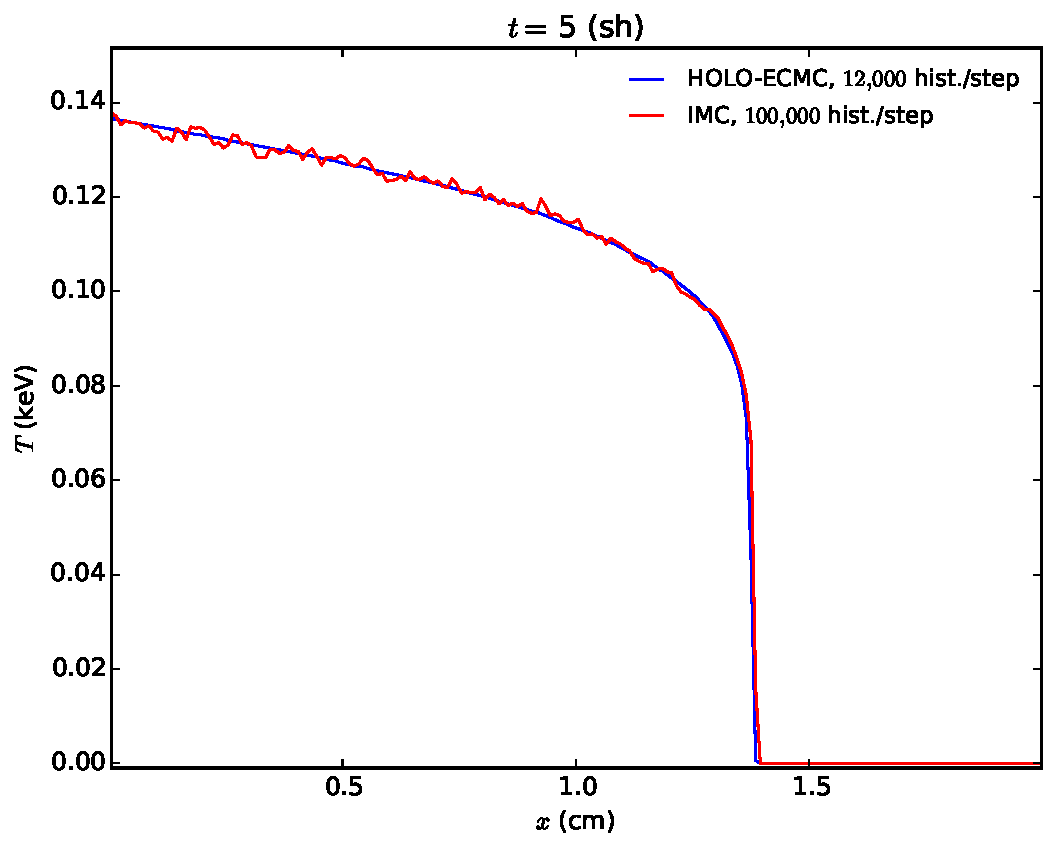
\includegraphics[width=0.5799\textwidth]{marshak_200_compare.pdf}
    \end{figure}
\end{frame}

%%%%%%%%%%%%%%%%%%%%%%%%%%%%%%%%%%%%%%%%%%%%%%%%%%%%%%%%%%%%%%%%%%%%%%%%%%%%%%%%%%%%%%%%%
\begin{frame}
    \frametitle{Two Material Problem, Comparison of Spatial Convergence}
    \begin{block}{}
        \begin{itemize}
            \item Same as Marshak Wave, but with constant opacities and an optically thin (left) and
                optically thick (right) region 
            \item Convergence of spatial mesh:
        \end{itemize}
    \end{block}
\begin{figure}
    \centering
    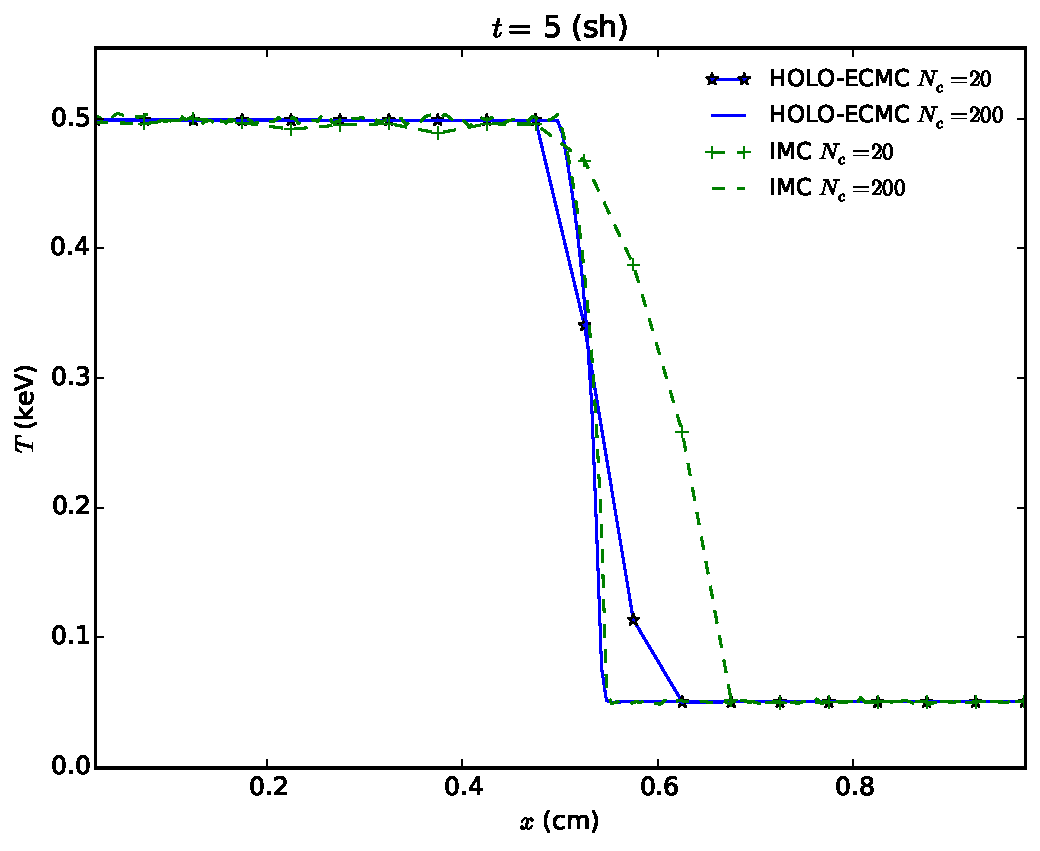
\includegraphics[width=0.5799\textwidth]{two_mat_conv.pdf}
\end{figure}

\end{frame}

\begin{frame}
    \frametitle{Comparison of statistical noise for standard and ECMC HO solvers}
    \begin{block}{}
    \begin{itemize}
        \item Two material problem
        \item One HO solve, with a \emph{fixed number of histories} per time step,
            for two different HO solvers: a
            comparison of
            \colr{ECMC} with 3 batches and standard MC (\colb{SMC}), as well as S$_2$
            solution
    \end{itemize}
    \end{block}
    \centering
    \begin{figure}
    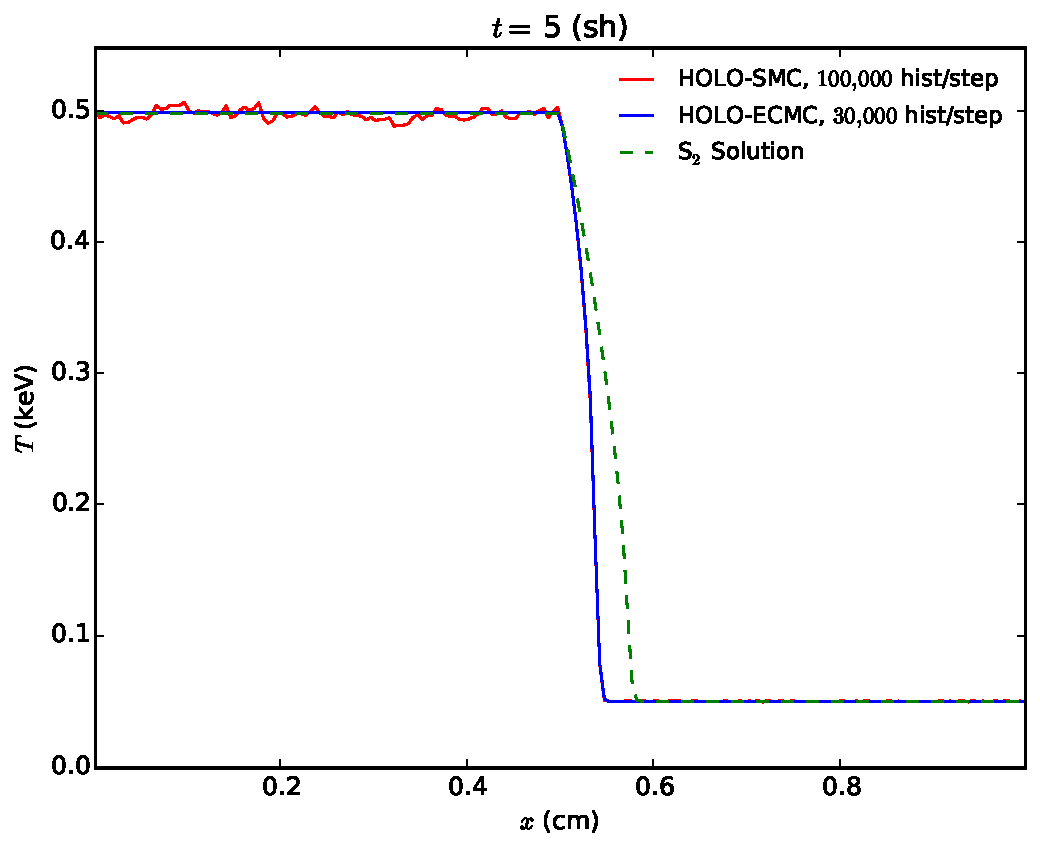
\includegraphics[width=0.5799\textwidth]{two_mat_ho_compare.pdf}
    \centering
    \end{figure}
\end{frame}

\section{Conclusions}
\subsection{}

%%%%%%%%%%%%%%%%%%%%%%%%%%%%%%%%%%%%%%%%%%%%%%%%%%%%%%%%%%%%%%%%%%%%%%%%%%%%%%%%%%%%%%%%%
\begin{frame}
    \frametitle{Current \& Future Development}
    \begin{itemize}
        \item Can accurately reproduce IMC results with HOLO method
        \begin{itemize}
            \item ECMC requires significantly less particles
            \item LO solver determines non-linear Material temperature distribution
            \item Linear shape within a cell mitigates teleportation error
            \item Very efficient for diffusive problems
        \end{itemize}
    \item Currently developing strategies for dealing with unresolvable solutions
    \item Future work will be to implement in 2 spatial dimensions to demonstrate the
        elimination of ray effects
    \end{itemize}
\end{frame}

\date{}
\begin{frame}
    \frametitle{{\LARGE\coly{Questions?}}}
    \vspace{-0.21in}
    \titlepage \vspace{-0.2113in}
\end{frame}

\appendix
\newcounter{finalframe}
\setcounter{finalframe}{\value{framenumber}}

\title{Backup Slides}
\author{}
\date{}

\begin{frame}
    \titlepage
\end{frame}


\begin{frame}
    \frametitle{ECMC procedure}
    {
    \begin{block}{Algorithm}
    \begin{enumerate}
        \item Intialize $\tilde I^{n+1,(0)}:=\tilde I^{n}$
        \item Using Monte Carlo, solve $\epsilon^{(m)} = \B L^{-1} \tilde r^{(m)}$
            \begin{itemize}
                \item Use volumetric tallies, weighted with $x$ and $\mu$ basis moments time $\psi$ to construct LD
                    $\tilde\epsilon^{(m)}(x,\mu)$ over the current space-angle mesh
            \end{itemize}
        \item $\tilde \psi^{(j+1)} = \tilde \psi^{(m)} + \tilde \epsilon^{(m)}$
        \item \textbf{IF} error stagnation:
            \begin{itemize}
                \item Refine mesh based on relative jump error in $\tilde \psi(x,\mu)$
            \end{itemize}
        \item Repeat 2-4 until $\| \tilde \epsilon \|_2 < \textsf{tol}\times
            \|\psi\|_2$
    \end{enumerate}
    \end{block}
}
\end{frame}

\begin{frame}
    \frametitle{HOLO Algorithm}
    {
    \begin{block}{Algorithm}
        \begin{enumerate}
            \item Initialize $\mom{\mu}^{\pm}$ parameters to S$_2$
            \item Solve LO system using power iteration
            \item Build $q^{LD}$ for HO solver, and set $\tilde{\psi}$ to latest
                HO estimate
                on coarsest $x$--$\mu$ mesh
            \item Solve $\tilde \psi(x,\mu) = \B L^{-1}q^{LO}$ using ECMC
            \item Compute new $\mom{\mu}^\pm$ parameters using $\tilde \psi^{HO}$ over LO mesh
            \item Repeat 2-5 until $\underline \Phi^{LO}$ is converged
        \end{enumerate}

    \begin{itemize}
        \item Use adaptive convergence criteria
    \end{itemize}
    \end{block}
}
\end{frame}

\begin{frame}
    \frametitle{LO System}
    \begin{itemize}
        \item Taking moments of TE yields \colb{4 equations}, per cell $i$, e.g.
\begin{multline}\label{lo_tran}
    -2{\mu}_{i-1/2}^{n+1,+} \phi_{i-1/2}^{n+1,+} + \cur {\mu}_{L,i}^{n+1,+}
  \mom{\phi}_{L,i}^{n+1,+}
  +  \cur\mu_{R,i}^{n+1,+}
  \mom{\phi}_{R,i}^{n+1,+} +  \left(\sigma_t^{n+1}+\frac{1}{c \Delta t} \right) h_i 
  \mom{\phi}_{L,i}^{n+1,+} \\-  \frac{\sigma_s h_i}{2} \left( \mom{\phi}_{L,i}^{n+1,+} +
  \mom\phi_{L,i}^{n+1,-}\right) = \frac{h_i}{2} \mom{\sigma_a^{n+1} a c T^{n+1,4}}_{L,i} +
  \frac{h_i}{c\Delta t}\mom{\phi}_{L,i}^{n,+},
\end{multline}
        \item Cell unknowns: $\mom{\phi}_{L,i}^{+}$, $\mom{\phi}_{R,i}^{+}$,
        $\mom{\phi}_{L,i}^{-}$, $\mom{\phi}_{R,i}^{-}$, $T_L$, $T_R$

    \item Need \colb{angular} consistency terms  and spatial closure
        (LD)
    \end{itemize}

\end{frame}

\begin{frame}
    \frametitle{Solving LO System with Newton's Method}
    \begin{block}{}
    \begin{itemize}
        \item Linearization: $\displaystyle \u B(T^{n+1}) = \u B(T^*) + \left(T^{n+1} -
                T^*\right) \pderiv{\u B}{t}\bigg|_{t^*}$
        \vspace{-0.15in}
        \item Modified system
            \begin{gather*}
                \displaystyle \left[\B  D(\mu^\pm) - \sigma_a^*(1-f^*) \right]\underline
                \Phi^{n+1}  = f^* \u B(T^*) + \frac{ \underline \Phi^n}{c\Delta t} \\
                \boxed{\hat{ \B  D }\Phi^{n+1} = \underline Q}
            \end{gather*}
        \vspace{-0.07in}
        \begin{center}
         $\displaystyle f = \left( 1 + \sigma_a^*c \Delta t \frac{4aT^{*3}}{\rho
            c_v} \right)^{-1}$  \hspace{0.3in}
         $\displaystyle T_i^* = \frac{T^{*}_{L,i}+T^{*}_{R,i}}{2}$
     \end{center}
 \item Equation for $T^{n+1}$ based on linearization that is conservative
 \item Converge $T^{n+1}$ and $\mom{\phi}$ with Newton Iterations
     \begin{itemize}
 \item Spatial representation can result in negative temperatures
     \end{itemize}
 \end{itemize}
 \end{block}
\end{frame}

\setcounter{framenumber}{\value{finalframe}}
\end{document}
